\documentclass[]{article}
\usepackage{lmodern}
\usepackage{amssymb,amsmath}
\usepackage{ifxetex,ifluatex}
\usepackage{fixltx2e} % provides \textsubscript
\ifnum 0\ifxetex 1\fi\ifluatex 1\fi=0 % if pdftex
  \usepackage[T1]{fontenc}
  \usepackage[utf8]{inputenc}
\else % if luatex or xelatex
  \ifxetex
    \usepackage{mathspec}
  \else
    \usepackage{fontspec}
  \fi
  \defaultfontfeatures{Ligatures=TeX,Scale=MatchLowercase}
\fi
% use upquote if available, for straight quotes in verbatim environments
\IfFileExists{upquote.sty}{\usepackage{upquote}}{}
% use microtype if available
\IfFileExists{microtype.sty}{%
\usepackage{microtype}
\UseMicrotypeSet[protrusion]{basicmath} % disable protrusion for tt fonts
}{}
\usepackage[margin=1in]{geometry}
\usepackage{hyperref}
\hypersetup{unicode=true,
            pdfborder={0 0 0},
            breaklinks=true}
\urlstyle{same}  % don't use monospace font for urls
\usepackage{color}
\usepackage{fancyvrb}
\newcommand{\VerbBar}{|}
\newcommand{\VERB}{\Verb[commandchars=\\\{\}]}
\DefineVerbatimEnvironment{Highlighting}{Verbatim}{commandchars=\\\{\}}
% Add ',fontsize=\small' for more characters per line
\usepackage{framed}
\definecolor{shadecolor}{RGB}{248,248,248}
\newenvironment{Shaded}{\begin{snugshade}}{\end{snugshade}}
\newcommand{\KeywordTok}[1]{\textcolor[rgb]{0.13,0.29,0.53}{\textbf{#1}}}
\newcommand{\DataTypeTok}[1]{\textcolor[rgb]{0.13,0.29,0.53}{#1}}
\newcommand{\DecValTok}[1]{\textcolor[rgb]{0.00,0.00,0.81}{#1}}
\newcommand{\BaseNTok}[1]{\textcolor[rgb]{0.00,0.00,0.81}{#1}}
\newcommand{\FloatTok}[1]{\textcolor[rgb]{0.00,0.00,0.81}{#1}}
\newcommand{\ConstantTok}[1]{\textcolor[rgb]{0.00,0.00,0.00}{#1}}
\newcommand{\CharTok}[1]{\textcolor[rgb]{0.31,0.60,0.02}{#1}}
\newcommand{\SpecialCharTok}[1]{\textcolor[rgb]{0.00,0.00,0.00}{#1}}
\newcommand{\StringTok}[1]{\textcolor[rgb]{0.31,0.60,0.02}{#1}}
\newcommand{\VerbatimStringTok}[1]{\textcolor[rgb]{0.31,0.60,0.02}{#1}}
\newcommand{\SpecialStringTok}[1]{\textcolor[rgb]{0.31,0.60,0.02}{#1}}
\newcommand{\ImportTok}[1]{#1}
\newcommand{\CommentTok}[1]{\textcolor[rgb]{0.56,0.35,0.01}{\textit{#1}}}
\newcommand{\DocumentationTok}[1]{\textcolor[rgb]{0.56,0.35,0.01}{\textbf{\textit{#1}}}}
\newcommand{\AnnotationTok}[1]{\textcolor[rgb]{0.56,0.35,0.01}{\textbf{\textit{#1}}}}
\newcommand{\CommentVarTok}[1]{\textcolor[rgb]{0.56,0.35,0.01}{\textbf{\textit{#1}}}}
\newcommand{\OtherTok}[1]{\textcolor[rgb]{0.56,0.35,0.01}{#1}}
\newcommand{\FunctionTok}[1]{\textcolor[rgb]{0.00,0.00,0.00}{#1}}
\newcommand{\VariableTok}[1]{\textcolor[rgb]{0.00,0.00,0.00}{#1}}
\newcommand{\ControlFlowTok}[1]{\textcolor[rgb]{0.13,0.29,0.53}{\textbf{#1}}}
\newcommand{\OperatorTok}[1]{\textcolor[rgb]{0.81,0.36,0.00}{\textbf{#1}}}
\newcommand{\BuiltInTok}[1]{#1}
\newcommand{\ExtensionTok}[1]{#1}
\newcommand{\PreprocessorTok}[1]{\textcolor[rgb]{0.56,0.35,0.01}{\textit{#1}}}
\newcommand{\AttributeTok}[1]{\textcolor[rgb]{0.77,0.63,0.00}{#1}}
\newcommand{\RegionMarkerTok}[1]{#1}
\newcommand{\InformationTok}[1]{\textcolor[rgb]{0.56,0.35,0.01}{\textbf{\textit{#1}}}}
\newcommand{\WarningTok}[1]{\textcolor[rgb]{0.56,0.35,0.01}{\textbf{\textit{#1}}}}
\newcommand{\AlertTok}[1]{\textcolor[rgb]{0.94,0.16,0.16}{#1}}
\newcommand{\ErrorTok}[1]{\textcolor[rgb]{0.64,0.00,0.00}{\textbf{#1}}}
\newcommand{\NormalTok}[1]{#1}
\usepackage{graphicx,grffile}
\makeatletter
\def\maxwidth{\ifdim\Gin@nat@width>\linewidth\linewidth\else\Gin@nat@width\fi}
\def\maxheight{\ifdim\Gin@nat@height>\textheight\textheight\else\Gin@nat@height\fi}
\makeatother
% Scale images if necessary, so that they will not overflow the page
% margins by default, and it is still possible to overwrite the defaults
% using explicit options in \includegraphics[width, height, ...]{}
\setkeys{Gin}{width=\maxwidth,height=\maxheight,keepaspectratio}
\IfFileExists{parskip.sty}{%
\usepackage{parskip}
}{% else
\setlength{\parindent}{0pt}
\setlength{\parskip}{6pt plus 2pt minus 1pt}
}
\setlength{\emergencystretch}{3em}  % prevent overfull lines
\providecommand{\tightlist}{%
  \setlength{\itemsep}{0pt}\setlength{\parskip}{0pt}}
\setcounter{secnumdepth}{0}
% Redefines (sub)paragraphs to behave more like sections
\ifx\paragraph\undefined\else
\let\oldparagraph\paragraph
\renewcommand{\paragraph}[1]{\oldparagraph{#1}\mbox{}}
\fi
\ifx\subparagraph\undefined\else
\let\oldsubparagraph\subparagraph
\renewcommand{\subparagraph}[1]{\oldsubparagraph{#1}\mbox{}}
\fi

%%% Use protect on footnotes to avoid problems with footnotes in titles
\let\rmarkdownfootnote\footnote%
\def\footnote{\protect\rmarkdownfootnote}

%%% Change title format to be more compact
\usepackage{titling}

% Create subtitle command for use in maketitle
\newcommand{\subtitle}[1]{
  \posttitle{
    \begin{center}\large#1\end{center}
    }
}

\setlength{\droptitle}{-2em}

  \title{}
    \pretitle{\vspace{\droptitle}}
  \posttitle{}
    \author{}
    \preauthor{}\postauthor{}
    \date{}
    \predate{}\postdate{}
  

\begin{document}

\begin{Shaded}
\begin{Highlighting}[]
\NormalTok{knitr}\OperatorTok{::}\NormalTok{opts_chunk}\OperatorTok{$}\KeywordTok{set}\NormalTok{(}\DataTypeTok{echo =} \OtherTok{TRUE}\NormalTok{)}
\NormalTok{nsims <-}\StringTok{ }\DecValTok{10} \CommentTok{#set number of simulations}
\KeywordTok{library}\NormalTok{(mvtnorm)}
\KeywordTok{library}\NormalTok{(MASS)}
\KeywordTok{library}\NormalTok{(afex)}
\end{Highlighting}
\end{Shaded}

\begin{verbatim}
## Loading required package: lme4
\end{verbatim}

\begin{verbatim}
## Loading required package: Matrix
\end{verbatim}

\begin{verbatim}
## ************
## Welcome to afex. For support visit: http://afex.singmann.science/
\end{verbatim}

\begin{verbatim}
## - Functions for ANOVAs: aov_car(), aov_ez(), and aov_4()
## - Methods for calculating p-values with mixed(): 'KR', 'S', 'LRT', and 'PB'
## - 'afex_aov' and 'mixed' objects can be passed to emmeans() for follow-up tests
## - NEWS: library('emmeans') now needs to be called explicitly!
## - Get and set global package options with: afex_options()
## - Set orthogonal sum-to-zero contrasts globally: set_sum_contrasts()
## - For example analyses see: browseVignettes("afex")
## ************
\end{verbatim}

\begin{verbatim}
## 
## Attaching package: 'afex'
\end{verbatim}

\begin{verbatim}
## The following object is masked from 'package:lme4':
## 
##     lmer
\end{verbatim}

\begin{Shaded}
\begin{Highlighting}[]
\KeywordTok{library}\NormalTok{(emmeans)}
\KeywordTok{library}\NormalTok{(ggplot2)}
\KeywordTok{library}\NormalTok{(gridExtra)}
\KeywordTok{library}\NormalTok{(reshape2)}
\KeywordTok{library}\NormalTok{(pwr)}

\CommentTok{# Install functions from GitHub by running the code below:}
\KeywordTok{source}\NormalTok{(}\StringTok{"https://raw.githubusercontent.com/Lakens/ANOVA_power_simulation/master/ANOVA_design.R"}\NormalTok{)}
\KeywordTok{source}\NormalTok{(}\StringTok{"https://raw.githubusercontent.com/Lakens/ANOVA_power_simulation/master/ANOVA_power.R"}\NormalTok{)}
\KeywordTok{source}\NormalTok{(}\StringTok{"https://raw.githubusercontent.com/Lakens/ANOVA_power_simulation/master/helper_functions/power_oneway_between.R"}\NormalTok{)}
\KeywordTok{source}\NormalTok{(}\StringTok{"https://raw.githubusercontent.com/Lakens/ANOVA_power_simulation/master/helper_functions/power_oneway_within.R"}\NormalTok{)}
\KeywordTok{source}\NormalTok{(}\StringTok{"https://raw.githubusercontent.com/Lakens/ANOVA_power_simulation/master/helper_functions/power_twoway_between.R"}\NormalTok{)}
\KeywordTok{source}\NormalTok{(}\StringTok{"https://raw.githubusercontent.com/Lakens/ANOVA_power_simulation/master/helper_functions/power_2x2_within.R"}\NormalTok{)}
\KeywordTok{source}\NormalTok{(}\StringTok{"https://raw.githubusercontent.com/Lakens/ANOVA_power_simulation/master/helper_functions/plot_power_oneway_between.R"}\NormalTok{)}
\KeywordTok{source}\NormalTok{(}\StringTok{"https://raw.githubusercontent.com/Lakens/ANOVA_power_simulation/master/helper_functions/plot_power_oneway_within.R"}\NormalTok{)}
\KeywordTok{source}\NormalTok{(}\StringTok{"https://raw.githubusercontent.com/Lakens/ANOVA_power_simulation/master/helper_functions/plot_power_twoway_between.R"}\NormalTok{)}
\KeywordTok{source}\NormalTok{(}\StringTok{"https://raw.githubusercontent.com/Lakens/ANOVA_power_simulation/master/helper_functions/plot_power_2x2_within.R"}\NormalTok{)}
\end{Highlighting}
\end{Shaded}

\subsection{Power for Design
Variations}\label{power-for-design-variations}

Researchers might consider what the effects on the statistical power of
their design is, when they add participants. Participants can be added
to an additional condition, or to the existing design.

In a One-Way ANOVA adding a condition means, for example, going from a
1x2 to a 1x3 design. For example, in addition to a control and intensive
training condition, we add a light training condition.

\begin{Shaded}
\begin{Highlighting}[]
\NormalTok{string <-}\StringTok{ "2b"}
\NormalTok{n <-}\StringTok{ }\DecValTok{50}
\NormalTok{mu <-}\StringTok{ }\KeywordTok{c}\NormalTok{(}\DecValTok{80}\NormalTok{, }\DecValTok{86}\NormalTok{) }\CommentTok{#All means are equal - so there is no real difference.}
\NormalTok{sd <-}\StringTok{ }\DecValTok{10}
\NormalTok{r <-}\StringTok{ }\DecValTok{0} 
\NormalTok{p_adjust =}\StringTok{ "none"}
\NormalTok{labelnames <-}\StringTok{ }\KeywordTok{c}\NormalTok{(}\StringTok{"Condition"}\NormalTok{, }\StringTok{"control"}\NormalTok{, }\StringTok{"intensive_training"}\NormalTok{) }\CommentTok{#}

\NormalTok{design_result <-}\StringTok{ }\KeywordTok{ANOVA_design}\NormalTok{(}\DataTypeTok{string =}\NormalTok{ string,}
                   \DataTypeTok{n =}\NormalTok{ n, }
                   \DataTypeTok{mu =}\NormalTok{ mu, }
                   \DataTypeTok{sd =}\NormalTok{ sd, }
                   \DataTypeTok{r =}\NormalTok{ r, }
                   \DataTypeTok{p_adjust =}\NormalTok{ p_adjust,}
                   \DataTypeTok{labelnames =}\NormalTok{ labelnames)}
\end{Highlighting}
\end{Shaded}

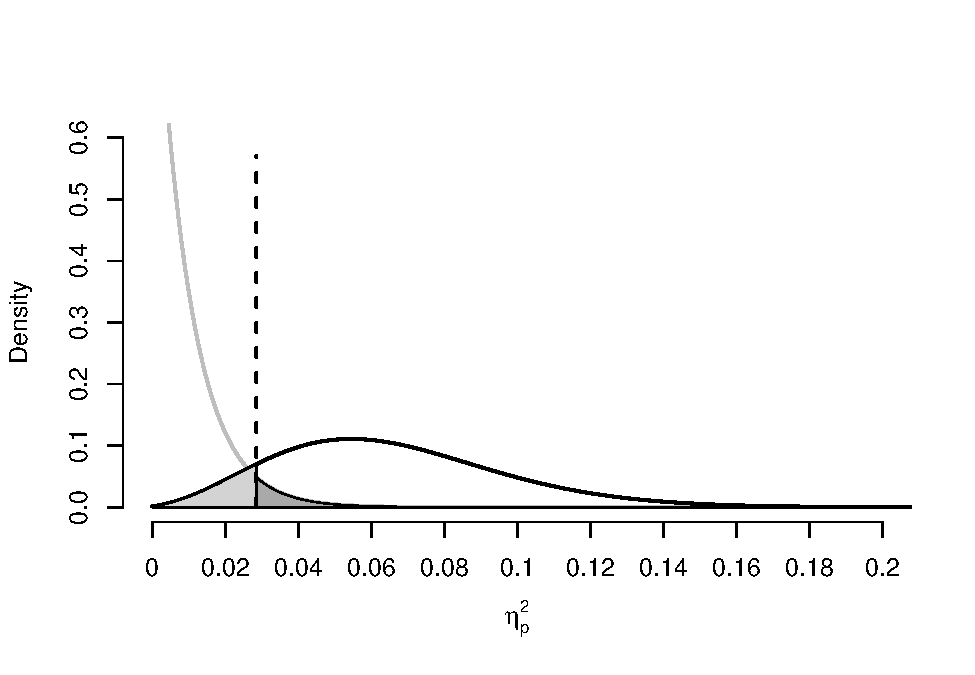
\includegraphics{4.5_power_for_design_variations_files/figure-latex/unnamed-chunk-1-1.pdf}

\begin{Shaded}
\begin{Highlighting}[]
\CommentTok{# Power for the given N in the design_result}
\KeywordTok{power_oneway_between}\NormalTok{(design_result)}\OperatorTok{$}\NormalTok{power}
\end{Highlighting}
\end{Shaded}

\begin{verbatim}
## [1] 0.8438754
\end{verbatim}

\begin{Shaded}
\begin{Highlighting}[]
\KeywordTok{power_oneway_between}\NormalTok{(design_result)}\OperatorTok{$}\NormalTok{Cohen_f}
\end{Highlighting}
\end{Shaded}

\begin{verbatim}
## [1] 0.3
\end{verbatim}

\begin{Shaded}
\begin{Highlighting}[]
\KeywordTok{power_oneway_between}\NormalTok{(design_result)}\OperatorTok{$}\NormalTok{eta_p_}\DecValTok{2}
\end{Highlighting}
\end{Shaded}

\begin{verbatim}
## [1] 0.08256881
\end{verbatim}

\begin{Shaded}
\begin{Highlighting}[]
\CommentTok{# Plot power curve (from 5 to 100)}
\KeywordTok{plot_power_oneway_between}\NormalTok{(design_result,}
                          \DataTypeTok{max_n =} \DecValTok{100}\NormalTok{)}\OperatorTok{$}\NormalTok{p1}
\end{Highlighting}
\end{Shaded}

\includegraphics{4.5_power_for_design_variations_files/figure-latex/unnamed-chunk-1-2.pdf}
\includegraphics{4.5_power_for_design_variations_files/figure-latex/unnamed-chunk-1-3.pdf}
\includegraphics{4.5_power_for_design_variations_files/figure-latex/unnamed-chunk-1-4.pdf}
\includegraphics{4.5_power_for_design_variations_files/figure-latex/unnamed-chunk-1-5.pdf}
\includegraphics{4.5_power_for_design_variations_files/figure-latex/unnamed-chunk-1-6.pdf}
\includegraphics{4.5_power_for_design_variations_files/figure-latex/unnamed-chunk-1-7.pdf}
\includegraphics{4.5_power_for_design_variations_files/figure-latex/unnamed-chunk-1-8.pdf}
\includegraphics{4.5_power_for_design_variations_files/figure-latex/unnamed-chunk-1-9.pdf}
\includegraphics{4.5_power_for_design_variations_files/figure-latex/unnamed-chunk-1-10.pdf}
\includegraphics{4.5_power_for_design_variations_files/figure-latex/unnamed-chunk-1-11.pdf}
\includegraphics{4.5_power_for_design_variations_files/figure-latex/unnamed-chunk-1-12.pdf}
\includegraphics{4.5_power_for_design_variations_files/figure-latex/unnamed-chunk-1-13.pdf}
\includegraphics{4.5_power_for_design_variations_files/figure-latex/unnamed-chunk-1-14.pdf}
\includegraphics{4.5_power_for_design_variations_files/figure-latex/unnamed-chunk-1-15.pdf}
\includegraphics{4.5_power_for_design_variations_files/figure-latex/unnamed-chunk-1-16.pdf}
\includegraphics{4.5_power_for_design_variations_files/figure-latex/unnamed-chunk-1-17.pdf}
\includegraphics{4.5_power_for_design_variations_files/figure-latex/unnamed-chunk-1-18.pdf}
\includegraphics{4.5_power_for_design_variations_files/figure-latex/unnamed-chunk-1-19.pdf}
\includegraphics{4.5_power_for_design_variations_files/figure-latex/unnamed-chunk-1-20.pdf}
\includegraphics{4.5_power_for_design_variations_files/figure-latex/unnamed-chunk-1-21.pdf}
\includegraphics{4.5_power_for_design_variations_files/figure-latex/unnamed-chunk-1-22.pdf}
\includegraphics{4.5_power_for_design_variations_files/figure-latex/unnamed-chunk-1-23.pdf}
\includegraphics{4.5_power_for_design_variations_files/figure-latex/unnamed-chunk-1-24.pdf}
\includegraphics{4.5_power_for_design_variations_files/figure-latex/unnamed-chunk-1-25.pdf}
\includegraphics{4.5_power_for_design_variations_files/figure-latex/unnamed-chunk-1-26.pdf}
\includegraphics{4.5_power_for_design_variations_files/figure-latex/unnamed-chunk-1-27.pdf}
\includegraphics{4.5_power_for_design_variations_files/figure-latex/unnamed-chunk-1-28.pdf}
\includegraphics{4.5_power_for_design_variations_files/figure-latex/unnamed-chunk-1-29.pdf}
\includegraphics{4.5_power_for_design_variations_files/figure-latex/unnamed-chunk-1-30.pdf}
\includegraphics{4.5_power_for_design_variations_files/figure-latex/unnamed-chunk-1-31.pdf}
\includegraphics{4.5_power_for_design_variations_files/figure-latex/unnamed-chunk-1-32.pdf}
\includegraphics{4.5_power_for_design_variations_files/figure-latex/unnamed-chunk-1-33.pdf}
\includegraphics{4.5_power_for_design_variations_files/figure-latex/unnamed-chunk-1-34.pdf}
\includegraphics{4.5_power_for_design_variations_files/figure-latex/unnamed-chunk-1-35.pdf}
\includegraphics{4.5_power_for_design_variations_files/figure-latex/unnamed-chunk-1-36.pdf}
\includegraphics{4.5_power_for_design_variations_files/figure-latex/unnamed-chunk-1-37.pdf}
\includegraphics{4.5_power_for_design_variations_files/figure-latex/unnamed-chunk-1-38.pdf}
\includegraphics{4.5_power_for_design_variations_files/figure-latex/unnamed-chunk-1-39.pdf}
\includegraphics{4.5_power_for_design_variations_files/figure-latex/unnamed-chunk-1-40.pdf}
\includegraphics{4.5_power_for_design_variations_files/figure-latex/unnamed-chunk-1-41.pdf}
\includegraphics{4.5_power_for_design_variations_files/figure-latex/unnamed-chunk-1-42.pdf}
\includegraphics{4.5_power_for_design_variations_files/figure-latex/unnamed-chunk-1-43.pdf}
\includegraphics{4.5_power_for_design_variations_files/figure-latex/unnamed-chunk-1-44.pdf}
\includegraphics{4.5_power_for_design_variations_files/figure-latex/unnamed-chunk-1-45.pdf}
\includegraphics{4.5_power_for_design_variations_files/figure-latex/unnamed-chunk-1-46.pdf}
\includegraphics{4.5_power_for_design_variations_files/figure-latex/unnamed-chunk-1-47.pdf}
\includegraphics{4.5_power_for_design_variations_files/figure-latex/unnamed-chunk-1-48.pdf}
\includegraphics{4.5_power_for_design_variations_files/figure-latex/unnamed-chunk-1-49.pdf}
\includegraphics{4.5_power_for_design_variations_files/figure-latex/unnamed-chunk-1-50.pdf}
\includegraphics{4.5_power_for_design_variations_files/figure-latex/unnamed-chunk-1-51.pdf}
\includegraphics{4.5_power_for_design_variations_files/figure-latex/unnamed-chunk-1-52.pdf}
\includegraphics{4.5_power_for_design_variations_files/figure-latex/unnamed-chunk-1-53.pdf}
\includegraphics{4.5_power_for_design_variations_files/figure-latex/unnamed-chunk-1-54.pdf}
\includegraphics{4.5_power_for_design_variations_files/figure-latex/unnamed-chunk-1-55.pdf}
\includegraphics{4.5_power_for_design_variations_files/figure-latex/unnamed-chunk-1-56.pdf}
\includegraphics{4.5_power_for_design_variations_files/figure-latex/unnamed-chunk-1-57.pdf}
\includegraphics{4.5_power_for_design_variations_files/figure-latex/unnamed-chunk-1-58.pdf}
\includegraphics{4.5_power_for_design_variations_files/figure-latex/unnamed-chunk-1-59.pdf}
\includegraphics{4.5_power_for_design_variations_files/figure-latex/unnamed-chunk-1-60.pdf}
\includegraphics{4.5_power_for_design_variations_files/figure-latex/unnamed-chunk-1-61.pdf}
\includegraphics{4.5_power_for_design_variations_files/figure-latex/unnamed-chunk-1-62.pdf}
\includegraphics{4.5_power_for_design_variations_files/figure-latex/unnamed-chunk-1-63.pdf}
\includegraphics{4.5_power_for_design_variations_files/figure-latex/unnamed-chunk-1-64.pdf}
\includegraphics{4.5_power_for_design_variations_files/figure-latex/unnamed-chunk-1-65.pdf}
\includegraphics{4.5_power_for_design_variations_files/figure-latex/unnamed-chunk-1-66.pdf}
\includegraphics{4.5_power_for_design_variations_files/figure-latex/unnamed-chunk-1-67.pdf}
\includegraphics{4.5_power_for_design_variations_files/figure-latex/unnamed-chunk-1-68.pdf}
\includegraphics{4.5_power_for_design_variations_files/figure-latex/unnamed-chunk-1-69.pdf}
\includegraphics{4.5_power_for_design_variations_files/figure-latex/unnamed-chunk-1-70.pdf}
\includegraphics{4.5_power_for_design_variations_files/figure-latex/unnamed-chunk-1-71.pdf}
\includegraphics{4.5_power_for_design_variations_files/figure-latex/unnamed-chunk-1-72.pdf}
\includegraphics{4.5_power_for_design_variations_files/figure-latex/unnamed-chunk-1-73.pdf}
\includegraphics{4.5_power_for_design_variations_files/figure-latex/unnamed-chunk-1-74.pdf}
\includegraphics{4.5_power_for_design_variations_files/figure-latex/unnamed-chunk-1-75.pdf}
\includegraphics{4.5_power_for_design_variations_files/figure-latex/unnamed-chunk-1-76.pdf}
\includegraphics{4.5_power_for_design_variations_files/figure-latex/unnamed-chunk-1-77.pdf}
\includegraphics{4.5_power_for_design_variations_files/figure-latex/unnamed-chunk-1-78.pdf}
\includegraphics{4.5_power_for_design_variations_files/figure-latex/unnamed-chunk-1-79.pdf}
\includegraphics{4.5_power_for_design_variations_files/figure-latex/unnamed-chunk-1-80.pdf}
\includegraphics{4.5_power_for_design_variations_files/figure-latex/unnamed-chunk-1-81.pdf}
\includegraphics{4.5_power_for_design_variations_files/figure-latex/unnamed-chunk-1-82.pdf}
\includegraphics{4.5_power_for_design_variations_files/figure-latex/unnamed-chunk-1-83.pdf}
\includegraphics{4.5_power_for_design_variations_files/figure-latex/unnamed-chunk-1-84.pdf}
\includegraphics{4.5_power_for_design_variations_files/figure-latex/unnamed-chunk-1-85.pdf}
\includegraphics{4.5_power_for_design_variations_files/figure-latex/unnamed-chunk-1-86.pdf}
\includegraphics{4.5_power_for_design_variations_files/figure-latex/unnamed-chunk-1-87.pdf}
\includegraphics{4.5_power_for_design_variations_files/figure-latex/unnamed-chunk-1-88.pdf}
\includegraphics{4.5_power_for_design_variations_files/figure-latex/unnamed-chunk-1-89.pdf}
\includegraphics{4.5_power_for_design_variations_files/figure-latex/unnamed-chunk-1-90.pdf}
\includegraphics{4.5_power_for_design_variations_files/figure-latex/unnamed-chunk-1-91.pdf}
\includegraphics{4.5_power_for_design_variations_files/figure-latex/unnamed-chunk-1-92.pdf}
\includegraphics{4.5_power_for_design_variations_files/figure-latex/unnamed-chunk-1-93.pdf}
\includegraphics{4.5_power_for_design_variations_files/figure-latex/unnamed-chunk-1-94.pdf}
\includegraphics{4.5_power_for_design_variations_files/figure-latex/unnamed-chunk-1-95.pdf}
\includegraphics{4.5_power_for_design_variations_files/figure-latex/unnamed-chunk-1-96.pdf}
\includegraphics{4.5_power_for_design_variations_files/figure-latex/unnamed-chunk-1-97.pdf}
\includegraphics{4.5_power_for_design_variations_files/figure-latex/unnamed-chunk-1-98.pdf}

\begin{Shaded}
\begin{Highlighting}[]
\KeywordTok{ANOVA_power}\NormalTok{(design_result, }\DataTypeTok{nsims =}\NormalTok{ nsims)}
\end{Highlighting}
\end{Shaded}

\begin{verbatim}
## Power and Effect sizes for ANOVA tests
##                 power effect size
## anova_Condition    80      0.1036
## 
## Power and Effect sizes for contrasts
##                                                  power effect size
## p_Condition_control_Condition_intensive_training    80      0.5839
\end{verbatim}

We now addd a condition. Let's assume the `light training' condition
falls in between the other two means.

\begin{Shaded}
\begin{Highlighting}[]
\NormalTok{string <-}\StringTok{ "3b"}
\NormalTok{n <-}\StringTok{ }\DecValTok{50}
\NormalTok{mu <-}\StringTok{ }\KeywordTok{c}\NormalTok{(}\DecValTok{80}\NormalTok{, }\DecValTok{83}\NormalTok{, }\DecValTok{86}\NormalTok{) }\CommentTok{#All means are equal - so there is no real difference.}
\NormalTok{sd <-}\StringTok{ }\DecValTok{10}
\NormalTok{r <-}\StringTok{ }\DecValTok{0} 
\NormalTok{p_adjust =}\StringTok{ "none"}
\NormalTok{labelnames <-}\StringTok{ }\KeywordTok{c}\NormalTok{(}\StringTok{"Condition"}\NormalTok{, }\StringTok{"control"}\NormalTok{, }\StringTok{"light_training"}\NormalTok{, }\StringTok{"intensive_training"}\NormalTok{) }

\NormalTok{design_result <-}\StringTok{ }\KeywordTok{ANOVA_design}\NormalTok{(}\DataTypeTok{string =}\NormalTok{ string,}
                   \DataTypeTok{n =}\NormalTok{ n, }
                   \DataTypeTok{mu =}\NormalTok{ mu, }
                   \DataTypeTok{sd =}\NormalTok{ sd, }
                   \DataTypeTok{r =}\NormalTok{ r, }
                   \DataTypeTok{p_adjust =}\NormalTok{ p_adjust,}
                   \DataTypeTok{labelnames =}\NormalTok{ labelnames)}
\end{Highlighting}
\end{Shaded}

\includegraphics{4.5_power_for_design_variations_files/figure-latex/unnamed-chunk-2-1.pdf}

\begin{Shaded}
\begin{Highlighting}[]
\CommentTok{# Power for the given N in the design_result}
\KeywordTok{power_oneway_between}\NormalTok{(design_result)}\OperatorTok{$}\NormalTok{power}
\end{Highlighting}
\end{Shaded}

\begin{verbatim}
## [1] 0.7616545
\end{verbatim}

\begin{Shaded}
\begin{Highlighting}[]
\KeywordTok{power_oneway_between}\NormalTok{(design_result)}\OperatorTok{$}\NormalTok{Cohen_f}
\end{Highlighting}
\end{Shaded}

\begin{verbatim}
## [1] 0.244949
\end{verbatim}

\begin{Shaded}
\begin{Highlighting}[]
\KeywordTok{power_oneway_between}\NormalTok{(design_result)}\OperatorTok{$}\NormalTok{eta_p_}\DecValTok{2}
\end{Highlighting}
\end{Shaded}

\begin{verbatim}
## [1] 0.05660377
\end{verbatim}

\begin{Shaded}
\begin{Highlighting}[]
\CommentTok{# Plot power curve (from 5 to 100)}
\KeywordTok{plot_power_oneway_between}\NormalTok{(design_result,}
                          \DataTypeTok{max_n =} \DecValTok{100}\NormalTok{)}\OperatorTok{$}\NormalTok{p1}
\end{Highlighting}
\end{Shaded}

\includegraphics{4.5_power_for_design_variations_files/figure-latex/unnamed-chunk-2-2.pdf}
\includegraphics{4.5_power_for_design_variations_files/figure-latex/unnamed-chunk-2-3.pdf}
\includegraphics{4.5_power_for_design_variations_files/figure-latex/unnamed-chunk-2-4.pdf}
\includegraphics{4.5_power_for_design_variations_files/figure-latex/unnamed-chunk-2-5.pdf}
\includegraphics{4.5_power_for_design_variations_files/figure-latex/unnamed-chunk-2-6.pdf}
\includegraphics{4.5_power_for_design_variations_files/figure-latex/unnamed-chunk-2-7.pdf}
\includegraphics{4.5_power_for_design_variations_files/figure-latex/unnamed-chunk-2-8.pdf}
\includegraphics{4.5_power_for_design_variations_files/figure-latex/unnamed-chunk-2-9.pdf}
\includegraphics{4.5_power_for_design_variations_files/figure-latex/unnamed-chunk-2-10.pdf}
\includegraphics{4.5_power_for_design_variations_files/figure-latex/unnamed-chunk-2-11.pdf}
\includegraphics{4.5_power_for_design_variations_files/figure-latex/unnamed-chunk-2-12.pdf}
\includegraphics{4.5_power_for_design_variations_files/figure-latex/unnamed-chunk-2-13.pdf}
\includegraphics{4.5_power_for_design_variations_files/figure-latex/unnamed-chunk-2-14.pdf}
\includegraphics{4.5_power_for_design_variations_files/figure-latex/unnamed-chunk-2-15.pdf}
\includegraphics{4.5_power_for_design_variations_files/figure-latex/unnamed-chunk-2-16.pdf}
\includegraphics{4.5_power_for_design_variations_files/figure-latex/unnamed-chunk-2-17.pdf}
\includegraphics{4.5_power_for_design_variations_files/figure-latex/unnamed-chunk-2-18.pdf}
\includegraphics{4.5_power_for_design_variations_files/figure-latex/unnamed-chunk-2-19.pdf}
\includegraphics{4.5_power_for_design_variations_files/figure-latex/unnamed-chunk-2-20.pdf}
\includegraphics{4.5_power_for_design_variations_files/figure-latex/unnamed-chunk-2-21.pdf}
\includegraphics{4.5_power_for_design_variations_files/figure-latex/unnamed-chunk-2-22.pdf}
\includegraphics{4.5_power_for_design_variations_files/figure-latex/unnamed-chunk-2-23.pdf}
\includegraphics{4.5_power_for_design_variations_files/figure-latex/unnamed-chunk-2-24.pdf}
\includegraphics{4.5_power_for_design_variations_files/figure-latex/unnamed-chunk-2-25.pdf}
\includegraphics{4.5_power_for_design_variations_files/figure-latex/unnamed-chunk-2-26.pdf}
\includegraphics{4.5_power_for_design_variations_files/figure-latex/unnamed-chunk-2-27.pdf}
\includegraphics{4.5_power_for_design_variations_files/figure-latex/unnamed-chunk-2-28.pdf}
\includegraphics{4.5_power_for_design_variations_files/figure-latex/unnamed-chunk-2-29.pdf}
\includegraphics{4.5_power_for_design_variations_files/figure-latex/unnamed-chunk-2-30.pdf}
\includegraphics{4.5_power_for_design_variations_files/figure-latex/unnamed-chunk-2-31.pdf}
\includegraphics{4.5_power_for_design_variations_files/figure-latex/unnamed-chunk-2-32.pdf}
\includegraphics{4.5_power_for_design_variations_files/figure-latex/unnamed-chunk-2-33.pdf}
\includegraphics{4.5_power_for_design_variations_files/figure-latex/unnamed-chunk-2-34.pdf}
\includegraphics{4.5_power_for_design_variations_files/figure-latex/unnamed-chunk-2-35.pdf}
\includegraphics{4.5_power_for_design_variations_files/figure-latex/unnamed-chunk-2-36.pdf}
\includegraphics{4.5_power_for_design_variations_files/figure-latex/unnamed-chunk-2-37.pdf}
\includegraphics{4.5_power_for_design_variations_files/figure-latex/unnamed-chunk-2-38.pdf}
\includegraphics{4.5_power_for_design_variations_files/figure-latex/unnamed-chunk-2-39.pdf}
\includegraphics{4.5_power_for_design_variations_files/figure-latex/unnamed-chunk-2-40.pdf}
\includegraphics{4.5_power_for_design_variations_files/figure-latex/unnamed-chunk-2-41.pdf}
\includegraphics{4.5_power_for_design_variations_files/figure-latex/unnamed-chunk-2-42.pdf}
\includegraphics{4.5_power_for_design_variations_files/figure-latex/unnamed-chunk-2-43.pdf}
\includegraphics{4.5_power_for_design_variations_files/figure-latex/unnamed-chunk-2-44.pdf}
\includegraphics{4.5_power_for_design_variations_files/figure-latex/unnamed-chunk-2-45.pdf}
\includegraphics{4.5_power_for_design_variations_files/figure-latex/unnamed-chunk-2-46.pdf}
\includegraphics{4.5_power_for_design_variations_files/figure-latex/unnamed-chunk-2-47.pdf}
\includegraphics{4.5_power_for_design_variations_files/figure-latex/unnamed-chunk-2-48.pdf}
\includegraphics{4.5_power_for_design_variations_files/figure-latex/unnamed-chunk-2-49.pdf}
\includegraphics{4.5_power_for_design_variations_files/figure-latex/unnamed-chunk-2-50.pdf}
\includegraphics{4.5_power_for_design_variations_files/figure-latex/unnamed-chunk-2-51.pdf}
\includegraphics{4.5_power_for_design_variations_files/figure-latex/unnamed-chunk-2-52.pdf}
\includegraphics{4.5_power_for_design_variations_files/figure-latex/unnamed-chunk-2-53.pdf}
\includegraphics{4.5_power_for_design_variations_files/figure-latex/unnamed-chunk-2-54.pdf}
\includegraphics{4.5_power_for_design_variations_files/figure-latex/unnamed-chunk-2-55.pdf}
\includegraphics{4.5_power_for_design_variations_files/figure-latex/unnamed-chunk-2-56.pdf}
\includegraphics{4.5_power_for_design_variations_files/figure-latex/unnamed-chunk-2-57.pdf}
\includegraphics{4.5_power_for_design_variations_files/figure-latex/unnamed-chunk-2-58.pdf}
\includegraphics{4.5_power_for_design_variations_files/figure-latex/unnamed-chunk-2-59.pdf}
\includegraphics{4.5_power_for_design_variations_files/figure-latex/unnamed-chunk-2-60.pdf}
\includegraphics{4.5_power_for_design_variations_files/figure-latex/unnamed-chunk-2-61.pdf}
\includegraphics{4.5_power_for_design_variations_files/figure-latex/unnamed-chunk-2-62.pdf}
\includegraphics{4.5_power_for_design_variations_files/figure-latex/unnamed-chunk-2-63.pdf}
\includegraphics{4.5_power_for_design_variations_files/figure-latex/unnamed-chunk-2-64.pdf}
\includegraphics{4.5_power_for_design_variations_files/figure-latex/unnamed-chunk-2-65.pdf}
\includegraphics{4.5_power_for_design_variations_files/figure-latex/unnamed-chunk-2-66.pdf}
\includegraphics{4.5_power_for_design_variations_files/figure-latex/unnamed-chunk-2-67.pdf}
\includegraphics{4.5_power_for_design_variations_files/figure-latex/unnamed-chunk-2-68.pdf}
\includegraphics{4.5_power_for_design_variations_files/figure-latex/unnamed-chunk-2-69.pdf}
\includegraphics{4.5_power_for_design_variations_files/figure-latex/unnamed-chunk-2-70.pdf}
\includegraphics{4.5_power_for_design_variations_files/figure-latex/unnamed-chunk-2-71.pdf}
\includegraphics{4.5_power_for_design_variations_files/figure-latex/unnamed-chunk-2-72.pdf}
\includegraphics{4.5_power_for_design_variations_files/figure-latex/unnamed-chunk-2-73.pdf}
\includegraphics{4.5_power_for_design_variations_files/figure-latex/unnamed-chunk-2-74.pdf}
\includegraphics{4.5_power_for_design_variations_files/figure-latex/unnamed-chunk-2-75.pdf}
\includegraphics{4.5_power_for_design_variations_files/figure-latex/unnamed-chunk-2-76.pdf}
\includegraphics{4.5_power_for_design_variations_files/figure-latex/unnamed-chunk-2-77.pdf}
\includegraphics{4.5_power_for_design_variations_files/figure-latex/unnamed-chunk-2-78.pdf}
\includegraphics{4.5_power_for_design_variations_files/figure-latex/unnamed-chunk-2-79.pdf}
\includegraphics{4.5_power_for_design_variations_files/figure-latex/unnamed-chunk-2-80.pdf}
\includegraphics{4.5_power_for_design_variations_files/figure-latex/unnamed-chunk-2-81.pdf}
\includegraphics{4.5_power_for_design_variations_files/figure-latex/unnamed-chunk-2-82.pdf}
\includegraphics{4.5_power_for_design_variations_files/figure-latex/unnamed-chunk-2-83.pdf}
\includegraphics{4.5_power_for_design_variations_files/figure-latex/unnamed-chunk-2-84.pdf}
\includegraphics{4.5_power_for_design_variations_files/figure-latex/unnamed-chunk-2-85.pdf}
\includegraphics{4.5_power_for_design_variations_files/figure-latex/unnamed-chunk-2-86.pdf}
\includegraphics{4.5_power_for_design_variations_files/figure-latex/unnamed-chunk-2-87.pdf}
\includegraphics{4.5_power_for_design_variations_files/figure-latex/unnamed-chunk-2-88.pdf}
\includegraphics{4.5_power_for_design_variations_files/figure-latex/unnamed-chunk-2-89.pdf}
\includegraphics{4.5_power_for_design_variations_files/figure-latex/unnamed-chunk-2-90.pdf}
\includegraphics{4.5_power_for_design_variations_files/figure-latex/unnamed-chunk-2-91.pdf}
\includegraphics{4.5_power_for_design_variations_files/figure-latex/unnamed-chunk-2-92.pdf}
\includegraphics{4.5_power_for_design_variations_files/figure-latex/unnamed-chunk-2-93.pdf}
\includegraphics{4.5_power_for_design_variations_files/figure-latex/unnamed-chunk-2-94.pdf}
\includegraphics{4.5_power_for_design_variations_files/figure-latex/unnamed-chunk-2-95.pdf}
\includegraphics{4.5_power_for_design_variations_files/figure-latex/unnamed-chunk-2-96.pdf}
\includegraphics{4.5_power_for_design_variations_files/figure-latex/unnamed-chunk-2-97.pdf}
\includegraphics{4.5_power_for_design_variations_files/figure-latex/unnamed-chunk-2-98.pdf}

We see that adding a condition that falls between the other two means
reduces our power. Let's instead assume that the `light training'
condition is not different from the control condition. In other words,
the mean we add is as extreme as one of the existing means.

\begin{Shaded}
\begin{Highlighting}[]
\NormalTok{string <-}\StringTok{ "3b"}
\NormalTok{n <-}\StringTok{ }\DecValTok{50}
\NormalTok{mu <-}\StringTok{ }\KeywordTok{c}\NormalTok{(}\DecValTok{80}\NormalTok{, }\DecValTok{80}\NormalTok{, }\DecValTok{86}\NormalTok{) }\CommentTok{#All means are equal - so there is no real difference.}
\NormalTok{sd <-}\StringTok{ }\DecValTok{10}
\NormalTok{r <-}\StringTok{ }\DecValTok{0} 
\NormalTok{p_adjust =}\StringTok{ "none"}
\NormalTok{labelnames <-}\StringTok{ }\KeywordTok{c}\NormalTok{(}\StringTok{"Condition"}\NormalTok{, }\StringTok{"control"}\NormalTok{, }\StringTok{"light_training"}\NormalTok{, }\StringTok{"intensive_training"}\NormalTok{) }

\NormalTok{design_result <-}\StringTok{ }\KeywordTok{ANOVA_design}\NormalTok{(}\DataTypeTok{string =}\NormalTok{ string,}
                   \DataTypeTok{n =}\NormalTok{ n, }
                   \DataTypeTok{mu =}\NormalTok{ mu, }
                   \DataTypeTok{sd =}\NormalTok{ sd, }
                   \DataTypeTok{r =}\NormalTok{ r, }
                   \DataTypeTok{p_adjust =}\NormalTok{ p_adjust,}
                   \DataTypeTok{labelnames =}\NormalTok{ labelnames)}
\end{Highlighting}
\end{Shaded}

\includegraphics{4.5_power_for_design_variations_files/figure-latex/unnamed-chunk-3-1.pdf}

\begin{Shaded}
\begin{Highlighting}[]
\CommentTok{# Power for the given N in the design_result}
\KeywordTok{power_oneway_between}\NormalTok{(design_result)}\OperatorTok{$}\NormalTok{power}
\end{Highlighting}
\end{Shaded}

\begin{verbatim}
## [1] 0.8762941
\end{verbatim}

\begin{Shaded}
\begin{Highlighting}[]
\KeywordTok{power_oneway_between}\NormalTok{(design_result)}\OperatorTok{$}\NormalTok{Cohen_f}
\end{Highlighting}
\end{Shaded}

\begin{verbatim}
## [1] 0.2828427
\end{verbatim}

\begin{Shaded}
\begin{Highlighting}[]
\KeywordTok{power_oneway_between}\NormalTok{(design_result)}\OperatorTok{$}\NormalTok{eta_p_}\DecValTok{2}
\end{Highlighting}
\end{Shaded}

\begin{verbatim}
## [1] 0.07407407
\end{verbatim}

\begin{Shaded}
\begin{Highlighting}[]
\CommentTok{# Plot power curve (from 5 to 100)}
\KeywordTok{plot_power_oneway_between}\NormalTok{(design_result,}
                          \DataTypeTok{max_n =} \DecValTok{100}\NormalTok{)}\OperatorTok{$}\NormalTok{p1}
\end{Highlighting}
\end{Shaded}

\includegraphics{4.5_power_for_design_variations_files/figure-latex/unnamed-chunk-3-2.pdf}
\includegraphics{4.5_power_for_design_variations_files/figure-latex/unnamed-chunk-3-3.pdf}
\includegraphics{4.5_power_for_design_variations_files/figure-latex/unnamed-chunk-3-4.pdf}
\includegraphics{4.5_power_for_design_variations_files/figure-latex/unnamed-chunk-3-5.pdf}
\includegraphics{4.5_power_for_design_variations_files/figure-latex/unnamed-chunk-3-6.pdf}
\includegraphics{4.5_power_for_design_variations_files/figure-latex/unnamed-chunk-3-7.pdf}
\includegraphics{4.5_power_for_design_variations_files/figure-latex/unnamed-chunk-3-8.pdf}
\includegraphics{4.5_power_for_design_variations_files/figure-latex/unnamed-chunk-3-9.pdf}
\includegraphics{4.5_power_for_design_variations_files/figure-latex/unnamed-chunk-3-10.pdf}
\includegraphics{4.5_power_for_design_variations_files/figure-latex/unnamed-chunk-3-11.pdf}
\includegraphics{4.5_power_for_design_variations_files/figure-latex/unnamed-chunk-3-12.pdf}
\includegraphics{4.5_power_for_design_variations_files/figure-latex/unnamed-chunk-3-13.pdf}
\includegraphics{4.5_power_for_design_variations_files/figure-latex/unnamed-chunk-3-14.pdf}
\includegraphics{4.5_power_for_design_variations_files/figure-latex/unnamed-chunk-3-15.pdf}
\includegraphics{4.5_power_for_design_variations_files/figure-latex/unnamed-chunk-3-16.pdf}
\includegraphics{4.5_power_for_design_variations_files/figure-latex/unnamed-chunk-3-17.pdf}
\includegraphics{4.5_power_for_design_variations_files/figure-latex/unnamed-chunk-3-18.pdf}
\includegraphics{4.5_power_for_design_variations_files/figure-latex/unnamed-chunk-3-19.pdf}
\includegraphics{4.5_power_for_design_variations_files/figure-latex/unnamed-chunk-3-20.pdf}
\includegraphics{4.5_power_for_design_variations_files/figure-latex/unnamed-chunk-3-21.pdf}
\includegraphics{4.5_power_for_design_variations_files/figure-latex/unnamed-chunk-3-22.pdf}
\includegraphics{4.5_power_for_design_variations_files/figure-latex/unnamed-chunk-3-23.pdf}
\includegraphics{4.5_power_for_design_variations_files/figure-latex/unnamed-chunk-3-24.pdf}
\includegraphics{4.5_power_for_design_variations_files/figure-latex/unnamed-chunk-3-25.pdf}
\includegraphics{4.5_power_for_design_variations_files/figure-latex/unnamed-chunk-3-26.pdf}
\includegraphics{4.5_power_for_design_variations_files/figure-latex/unnamed-chunk-3-27.pdf}
\includegraphics{4.5_power_for_design_variations_files/figure-latex/unnamed-chunk-3-28.pdf}
\includegraphics{4.5_power_for_design_variations_files/figure-latex/unnamed-chunk-3-29.pdf}
\includegraphics{4.5_power_for_design_variations_files/figure-latex/unnamed-chunk-3-30.pdf}
\includegraphics{4.5_power_for_design_variations_files/figure-latex/unnamed-chunk-3-31.pdf}
\includegraphics{4.5_power_for_design_variations_files/figure-latex/unnamed-chunk-3-32.pdf}
\includegraphics{4.5_power_for_design_variations_files/figure-latex/unnamed-chunk-3-33.pdf}
\includegraphics{4.5_power_for_design_variations_files/figure-latex/unnamed-chunk-3-34.pdf}
\includegraphics{4.5_power_for_design_variations_files/figure-latex/unnamed-chunk-3-35.pdf}
\includegraphics{4.5_power_for_design_variations_files/figure-latex/unnamed-chunk-3-36.pdf}
\includegraphics{4.5_power_for_design_variations_files/figure-latex/unnamed-chunk-3-37.pdf}
\includegraphics{4.5_power_for_design_variations_files/figure-latex/unnamed-chunk-3-38.pdf}
\includegraphics{4.5_power_for_design_variations_files/figure-latex/unnamed-chunk-3-39.pdf}
\includegraphics{4.5_power_for_design_variations_files/figure-latex/unnamed-chunk-3-40.pdf}
\includegraphics{4.5_power_for_design_variations_files/figure-latex/unnamed-chunk-3-41.pdf}
\includegraphics{4.5_power_for_design_variations_files/figure-latex/unnamed-chunk-3-42.pdf}
\includegraphics{4.5_power_for_design_variations_files/figure-latex/unnamed-chunk-3-43.pdf}
\includegraphics{4.5_power_for_design_variations_files/figure-latex/unnamed-chunk-3-44.pdf}
\includegraphics{4.5_power_for_design_variations_files/figure-latex/unnamed-chunk-3-45.pdf}
\includegraphics{4.5_power_for_design_variations_files/figure-latex/unnamed-chunk-3-46.pdf}
\includegraphics{4.5_power_for_design_variations_files/figure-latex/unnamed-chunk-3-47.pdf}
\includegraphics{4.5_power_for_design_variations_files/figure-latex/unnamed-chunk-3-48.pdf}
\includegraphics{4.5_power_for_design_variations_files/figure-latex/unnamed-chunk-3-49.pdf}
\includegraphics{4.5_power_for_design_variations_files/figure-latex/unnamed-chunk-3-50.pdf}
\includegraphics{4.5_power_for_design_variations_files/figure-latex/unnamed-chunk-3-51.pdf}
\includegraphics{4.5_power_for_design_variations_files/figure-latex/unnamed-chunk-3-52.pdf}
\includegraphics{4.5_power_for_design_variations_files/figure-latex/unnamed-chunk-3-53.pdf}
\includegraphics{4.5_power_for_design_variations_files/figure-latex/unnamed-chunk-3-54.pdf}
\includegraphics{4.5_power_for_design_variations_files/figure-latex/unnamed-chunk-3-55.pdf}
\includegraphics{4.5_power_for_design_variations_files/figure-latex/unnamed-chunk-3-56.pdf}
\includegraphics{4.5_power_for_design_variations_files/figure-latex/unnamed-chunk-3-57.pdf}
\includegraphics{4.5_power_for_design_variations_files/figure-latex/unnamed-chunk-3-58.pdf}
\includegraphics{4.5_power_for_design_variations_files/figure-latex/unnamed-chunk-3-59.pdf}
\includegraphics{4.5_power_for_design_variations_files/figure-latex/unnamed-chunk-3-60.pdf}
\includegraphics{4.5_power_for_design_variations_files/figure-latex/unnamed-chunk-3-61.pdf}
\includegraphics{4.5_power_for_design_variations_files/figure-latex/unnamed-chunk-3-62.pdf}
\includegraphics{4.5_power_for_design_variations_files/figure-latex/unnamed-chunk-3-63.pdf}
\includegraphics{4.5_power_for_design_variations_files/figure-latex/unnamed-chunk-3-64.pdf}
\includegraphics{4.5_power_for_design_variations_files/figure-latex/unnamed-chunk-3-65.pdf}
\includegraphics{4.5_power_for_design_variations_files/figure-latex/unnamed-chunk-3-66.pdf}
\includegraphics{4.5_power_for_design_variations_files/figure-latex/unnamed-chunk-3-67.pdf}
\includegraphics{4.5_power_for_design_variations_files/figure-latex/unnamed-chunk-3-68.pdf}
\includegraphics{4.5_power_for_design_variations_files/figure-latex/unnamed-chunk-3-69.pdf}
\includegraphics{4.5_power_for_design_variations_files/figure-latex/unnamed-chunk-3-70.pdf}
\includegraphics{4.5_power_for_design_variations_files/figure-latex/unnamed-chunk-3-71.pdf}
\includegraphics{4.5_power_for_design_variations_files/figure-latex/unnamed-chunk-3-72.pdf}
\includegraphics{4.5_power_for_design_variations_files/figure-latex/unnamed-chunk-3-73.pdf}
\includegraphics{4.5_power_for_design_variations_files/figure-latex/unnamed-chunk-3-74.pdf}
\includegraphics{4.5_power_for_design_variations_files/figure-latex/unnamed-chunk-3-75.pdf}
\includegraphics{4.5_power_for_design_variations_files/figure-latex/unnamed-chunk-3-76.pdf}
\includegraphics{4.5_power_for_design_variations_files/figure-latex/unnamed-chunk-3-77.pdf}
\includegraphics{4.5_power_for_design_variations_files/figure-latex/unnamed-chunk-3-78.pdf}
\includegraphics{4.5_power_for_design_variations_files/figure-latex/unnamed-chunk-3-79.pdf}
\includegraphics{4.5_power_for_design_variations_files/figure-latex/unnamed-chunk-3-80.pdf}
\includegraphics{4.5_power_for_design_variations_files/figure-latex/unnamed-chunk-3-81.pdf}
\includegraphics{4.5_power_for_design_variations_files/figure-latex/unnamed-chunk-3-82.pdf}
\includegraphics{4.5_power_for_design_variations_files/figure-latex/unnamed-chunk-3-83.pdf}
\includegraphics{4.5_power_for_design_variations_files/figure-latex/unnamed-chunk-3-84.pdf}
\includegraphics{4.5_power_for_design_variations_files/figure-latex/unnamed-chunk-3-85.pdf}
\includegraphics{4.5_power_for_design_variations_files/figure-latex/unnamed-chunk-3-86.pdf}
\includegraphics{4.5_power_for_design_variations_files/figure-latex/unnamed-chunk-3-87.pdf}
\includegraphics{4.5_power_for_design_variations_files/figure-latex/unnamed-chunk-3-88.pdf}
\includegraphics{4.5_power_for_design_variations_files/figure-latex/unnamed-chunk-3-89.pdf}
\includegraphics{4.5_power_for_design_variations_files/figure-latex/unnamed-chunk-3-90.pdf}
\includegraphics{4.5_power_for_design_variations_files/figure-latex/unnamed-chunk-3-91.pdf}
\includegraphics{4.5_power_for_design_variations_files/figure-latex/unnamed-chunk-3-92.pdf}
\includegraphics{4.5_power_for_design_variations_files/figure-latex/unnamed-chunk-3-93.pdf}
\includegraphics{4.5_power_for_design_variations_files/figure-latex/unnamed-chunk-3-94.pdf}
\includegraphics{4.5_power_for_design_variations_files/figure-latex/unnamed-chunk-3-95.pdf}
\includegraphics{4.5_power_for_design_variations_files/figure-latex/unnamed-chunk-3-96.pdf}
\includegraphics{4.5_power_for_design_variations_files/figure-latex/unnamed-chunk-3-97.pdf}
\includegraphics{4.5_power_for_design_variations_files/figure-latex/unnamed-chunk-3-98.pdf}

Now power has increased. This is not always true. The power is a
function of many factors in the design, incuding the effect size
(Cohen's f) and the total sample size (and the degrees of freedom and
number of groups). But as we will see below, as we keep adding
conditions, the power will reduce, even if initially, the power might
increase.

It helps to think of these different designs in terms of either partial
eta-squared, or Cohen's f (the one can easily be converted into the
other).

\begin{Shaded}
\begin{Highlighting}[]
\CommentTok{#Two groups}
\NormalTok{mu <-}\StringTok{ }\KeywordTok{c}\NormalTok{(}\DecValTok{80}\NormalTok{, }\DecValTok{86}\NormalTok{)}
\NormalTok{sd =}\StringTok{ }\DecValTok{10}
\NormalTok{n <-}\StringTok{ }\DecValTok{50} \CommentTok{#sample size per condition}
\NormalTok{mean_mat <-}\StringTok{ }\KeywordTok{t}\NormalTok{(}\KeywordTok{matrix}\NormalTok{(mu, }
                     \DataTypeTok{nrow =} \DecValTok{2}\NormalTok{,}
                     \DataTypeTok{ncol =} \DecValTok{1}\NormalTok{)) }\CommentTok{#Create a mean matrix}

\CommentTok{# Using the sweep function to remove rowmeans from the matrix}
\NormalTok{mean_mat_res <-}\StringTok{ }\KeywordTok{sweep}\NormalTok{(mean_mat,}\DecValTok{2}\NormalTok{, }\KeywordTok{rowMeans}\NormalTok{(mean_mat))   }
\NormalTok{mean_mat_res}
\end{Highlighting}
\end{Shaded}

\begin{verbatim}
##      [,1] [,2]
## [1,]   -3    3
\end{verbatim}

\begin{Shaded}
\begin{Highlighting}[]
\NormalTok{MS_a <-}\StringTok{ }\NormalTok{n }\OperatorTok{*}\StringTok{ }\NormalTok{(}\KeywordTok{sum}\NormalTok{(mean_mat_res}\OperatorTok{^}\DecValTok{2}\NormalTok{)}\OperatorTok{/}\NormalTok{(}\DecValTok{2}\OperatorTok{-}\DecValTok{1}\NormalTok{))}
\NormalTok{MS_a}
\end{Highlighting}
\end{Shaded}

\begin{verbatim}
## [1] 900
\end{verbatim}

\begin{Shaded}
\begin{Highlighting}[]
\NormalTok{SS_A <-}\StringTok{ }\NormalTok{n }\OperatorTok{*}\StringTok{ }\KeywordTok{sum}\NormalTok{(mean_mat_res}\OperatorTok{^}\DecValTok{2}\NormalTok{)}
\NormalTok{SS_A}
\end{Highlighting}
\end{Shaded}

\begin{verbatim}
## [1] 900
\end{verbatim}

\begin{Shaded}
\begin{Highlighting}[]
\NormalTok{MS_error <-}\StringTok{ }\NormalTok{sd}\OperatorTok{^}\DecValTok{2}
\NormalTok{MS_error}
\end{Highlighting}
\end{Shaded}

\begin{verbatim}
## [1] 100
\end{verbatim}

\begin{Shaded}
\begin{Highlighting}[]
\NormalTok{SS_error <-}\StringTok{ }\NormalTok{MS_error }\OperatorTok{*}\StringTok{ }\NormalTok{(n}\OperatorTok{*}\DecValTok{2}\NormalTok{) }
\NormalTok{SS_error}
\end{Highlighting}
\end{Shaded}

\begin{verbatim}
## [1] 10000
\end{verbatim}

\begin{Shaded}
\begin{Highlighting}[]
\NormalTok{eta_p_}\DecValTok{2}\NormalTok{ <-}\StringTok{ }\NormalTok{SS_A}\OperatorTok{/}\NormalTok{(SS_A}\OperatorTok{+}\NormalTok{SS_error)}
\NormalTok{eta_p_}\DecValTok{2}
\end{Highlighting}
\end{Shaded}

\begin{verbatim}
## [1] 0.08256881
\end{verbatim}

\begin{Shaded}
\begin{Highlighting}[]
\NormalTok{f_}\DecValTok{2}\NormalTok{ <-}\StringTok{ }\NormalTok{eta_p_}\DecValTok{2}\OperatorTok{/}\NormalTok{(}\DecValTok{1}\OperatorTok{-}\NormalTok{eta_p_}\DecValTok{2}\NormalTok{)}
\NormalTok{f_}\DecValTok{2}
\end{Highlighting}
\end{Shaded}

\begin{verbatim}
## [1] 0.09
\end{verbatim}

\begin{Shaded}
\begin{Highlighting}[]
\NormalTok{Cohen_f <-}\StringTok{ }\KeywordTok{sqrt}\NormalTok{(f_}\DecValTok{2}\NormalTok{)}
\NormalTok{Cohen_f}
\end{Highlighting}
\end{Shaded}

\begin{verbatim}
## [1] 0.3
\end{verbatim}

\begin{Shaded}
\begin{Highlighting}[]
\CommentTok{#Three groups}
\NormalTok{mu <-}\StringTok{ }\KeywordTok{c}\NormalTok{(}\DecValTok{80}\NormalTok{, }\DecValTok{83}\NormalTok{, }\DecValTok{86}\NormalTok{)}
\NormalTok{sd =}\StringTok{ }\DecValTok{10}
\NormalTok{n <-}\StringTok{ }\DecValTok{50}
\NormalTok{mean_mat <-}\StringTok{ }\KeywordTok{t}\NormalTok{(}\KeywordTok{matrix}\NormalTok{(mu, }
                     \DataTypeTok{nrow =} \DecValTok{3}\NormalTok{,}
                     \DataTypeTok{ncol =} \DecValTok{1}\NormalTok{)) }\CommentTok{#Create a mean matrix}

\CommentTok{# Using the sweep function to remove rowmeans from the matrix}
\NormalTok{mean_mat_res <-}\StringTok{ }\KeywordTok{sweep}\NormalTok{(mean_mat,}\DecValTok{2}\NormalTok{, }\KeywordTok{rowMeans}\NormalTok{(mean_mat))   }
\NormalTok{mean_mat_res}
\end{Highlighting}
\end{Shaded}

\begin{verbatim}
##      [,1] [,2] [,3]
## [1,]   -3    0    3
\end{verbatim}

\begin{Shaded}
\begin{Highlighting}[]
\NormalTok{MS_a <-}\StringTok{ }\NormalTok{n }\OperatorTok{*}\StringTok{ }\NormalTok{(}\KeywordTok{sum}\NormalTok{(mean_mat_res}\OperatorTok{^}\DecValTok{2}\NormalTok{)}\OperatorTok{/}\NormalTok{(}\DecValTok{3}\OperatorTok{-}\DecValTok{1}\NormalTok{))}
\NormalTok{MS_a}
\end{Highlighting}
\end{Shaded}

\begin{verbatim}
## [1] 450
\end{verbatim}

\begin{Shaded}
\begin{Highlighting}[]
\NormalTok{SS_A <-}\StringTok{ }\NormalTok{n }\OperatorTok{*}\StringTok{ }\KeywordTok{sum}\NormalTok{(mean_mat_res}\OperatorTok{^}\DecValTok{2}\NormalTok{)}
\NormalTok{SS_A}
\end{Highlighting}
\end{Shaded}

\begin{verbatim}
## [1] 900
\end{verbatim}

\begin{Shaded}
\begin{Highlighting}[]
\NormalTok{MS_error <-}\StringTok{ }\NormalTok{sd}\OperatorTok{^}\DecValTok{2}
\NormalTok{MS_error}
\end{Highlighting}
\end{Shaded}

\begin{verbatim}
## [1] 100
\end{verbatim}

\begin{Shaded}
\begin{Highlighting}[]
\NormalTok{SS_error <-}\StringTok{ }\NormalTok{MS_error }\OperatorTok{*}\StringTok{ }\NormalTok{(n}\OperatorTok{*}\DecValTok{3}\NormalTok{) }
\NormalTok{SS_error}
\end{Highlighting}
\end{Shaded}

\begin{verbatim}
## [1] 15000
\end{verbatim}

\begin{Shaded}
\begin{Highlighting}[]
\NormalTok{eta_p_}\DecValTok{2}\NormalTok{ <-}\StringTok{ }\NormalTok{SS_A}\OperatorTok{/}\NormalTok{(SS_A}\OperatorTok{+}\NormalTok{SS_error)}
\NormalTok{eta_p_}\DecValTok{2}
\end{Highlighting}
\end{Shaded}

\begin{verbatim}
## [1] 0.05660377
\end{verbatim}

\begin{Shaded}
\begin{Highlighting}[]
\NormalTok{f_}\DecValTok{2}\NormalTok{ <-}\StringTok{ }\NormalTok{eta_p_}\DecValTok{2}\OperatorTok{/}\NormalTok{(}\DecValTok{1}\OperatorTok{-}\NormalTok{eta_p_}\DecValTok{2}\NormalTok{)}
\NormalTok{f_}\DecValTok{2}
\end{Highlighting}
\end{Shaded}

\begin{verbatim}
## [1] 0.06
\end{verbatim}

\begin{Shaded}
\begin{Highlighting}[]
\NormalTok{Cohen_f <-}\StringTok{ }\KeywordTok{sqrt}\NormalTok{(f_}\DecValTok{2}\NormalTok{)}
\NormalTok{Cohen_f}
\end{Highlighting}
\end{Shaded}

\begin{verbatim}
## [1] 0.244949
\end{verbatim}

The SS\_A or the sum of squares for the main effect, is 900 for two
groups, and the SS\_error for the error term is 10000. When we add a
group, SS\_A is 900, and the SS\_error is 15000. Because the added
condition falls exactly on the grand mean (83), the sum of squared for
this extra group is 0. In other words, it does nothing to increase the
signal that there is a difference between groups. However, the sum of
squares for the error, which is a function of the total sample size, is
increased, which reduces the effect size. So, adding a condition that
falls on the grand mean reduces the power for the main effect of the
ANOVA. Obviously, adding such a group has other benefits, such as being
able to compare the two means to a new third condition.

We already saw that adding a condition that has a mean as extreme as one
of the existing groups also reduces the power. Let's again do the
calculations step by step when the extra group has a mean as extreme as
one of the two original conditions.

\begin{Shaded}
\begin{Highlighting}[]
\CommentTok{#Three groups}
\NormalTok{mu <-}\StringTok{ }\KeywordTok{c}\NormalTok{(}\DecValTok{80}\NormalTok{, }\DecValTok{80}\NormalTok{, }\DecValTok{86}\NormalTok{)}
\NormalTok{sd =}\StringTok{ }\DecValTok{10}
\NormalTok{n <-}\StringTok{ }\DecValTok{50}
\NormalTok{mean_mat <-}\StringTok{ }\KeywordTok{t}\NormalTok{(}\KeywordTok{matrix}\NormalTok{(mu, }
                     \DataTypeTok{nrow =} \DecValTok{3}\NormalTok{,}
                     \DataTypeTok{ncol =} \DecValTok{1}\NormalTok{)) }\CommentTok{#Create a mean matrix}

\CommentTok{# Using the sweep function to remove rowmeans from the matrix}
\NormalTok{mean_mat_res <-}\StringTok{ }\KeywordTok{sweep}\NormalTok{(mean_mat,}\DecValTok{2}\NormalTok{, }\KeywordTok{rowMeans}\NormalTok{(mean_mat))   }
\NormalTok{mean_mat_res}
\end{Highlighting}
\end{Shaded}

\begin{verbatim}
##      [,1] [,2] [,3]
## [1,]   -2   -2    4
\end{verbatim}

\begin{Shaded}
\begin{Highlighting}[]
\NormalTok{MS_a <-}\StringTok{ }\NormalTok{n }\OperatorTok{*}\StringTok{ }\NormalTok{(}\KeywordTok{sum}\NormalTok{(mean_mat_res}\OperatorTok{^}\DecValTok{2}\NormalTok{)}\OperatorTok{/}\NormalTok{(}\DecValTok{3}\OperatorTok{-}\DecValTok{1}\NormalTok{))}
\NormalTok{MS_a}
\end{Highlighting}
\end{Shaded}

\begin{verbatim}
## [1] 600
\end{verbatim}

\begin{Shaded}
\begin{Highlighting}[]
\NormalTok{SS_A <-}\StringTok{ }\NormalTok{n }\OperatorTok{*}\StringTok{ }\KeywordTok{sum}\NormalTok{(mean_mat_res}\OperatorTok{^}\DecValTok{2}\NormalTok{)}
\NormalTok{SS_A}
\end{Highlighting}
\end{Shaded}

\begin{verbatim}
## [1] 1200
\end{verbatim}

\begin{Shaded}
\begin{Highlighting}[]
\NormalTok{MS_error <-}\StringTok{ }\NormalTok{sd}\OperatorTok{^}\DecValTok{2}
\NormalTok{MS_error}
\end{Highlighting}
\end{Shaded}

\begin{verbatim}
## [1] 100
\end{verbatim}

\begin{Shaded}
\begin{Highlighting}[]
\NormalTok{SS_error <-}\StringTok{ }\NormalTok{MS_error }\OperatorTok{*}\StringTok{ }\NormalTok{(n}\OperatorTok{*}\DecValTok{3}\NormalTok{) }
\NormalTok{SS_error}
\end{Highlighting}
\end{Shaded}

\begin{verbatim}
## [1] 15000
\end{verbatim}

\begin{Shaded}
\begin{Highlighting}[]
\NormalTok{eta_p_}\DecValTok{2}\NormalTok{ <-}\StringTok{ }\NormalTok{SS_A}\OperatorTok{/}\NormalTok{(SS_A}\OperatorTok{+}\NormalTok{SS_error)}
\NormalTok{eta_p_}\DecValTok{2}
\end{Highlighting}
\end{Shaded}

\begin{verbatim}
## [1] 0.07407407
\end{verbatim}

\begin{Shaded}
\begin{Highlighting}[]
\NormalTok{f_}\DecValTok{2}\NormalTok{ <-}\StringTok{ }\NormalTok{eta_p_}\DecValTok{2}\OperatorTok{/}\NormalTok{(}\DecValTok{1}\OperatorTok{-}\NormalTok{eta_p_}\DecValTok{2}\NormalTok{)}
\NormalTok{f_}\DecValTok{2}
\end{Highlighting}
\end{Shaded}

\begin{verbatim}
## [1] 0.08
\end{verbatim}

\begin{Shaded}
\begin{Highlighting}[]
\NormalTok{Cohen_f <-}\StringTok{ }\KeywordTok{sqrt}\NormalTok{(f_}\DecValTok{2}\NormalTok{)}
\NormalTok{Cohen_f}
\end{Highlighting}
\end{Shaded}

\begin{verbatim}
## [1] 0.2828427
\end{verbatim}

We see the sum of squares of the error stays the same - 15000 - because
it is only determined by the standard error and the sample size, but not
by the differences in the means. This is an increase of 5000 compared to
the 2 group design. The sum of squares (the second component that
determines the size of partial eta-squared) increases, which increases
Cohen's f.

\section{Within Designs}\label{within-designs}

Now imagine our design described above was a within design. The means
and sd remain the same. We collect 50 participants (instead of 100, or
50 per group, for the between design). Let's first assume the two
samples are completely uncorrelated.

\begin{Shaded}
\begin{Highlighting}[]
\NormalTok{string <-}\StringTok{ "2w"}
\NormalTok{n <-}\StringTok{ }\DecValTok{50}
\NormalTok{mu <-}\StringTok{ }\KeywordTok{c}\NormalTok{(}\DecValTok{80}\NormalTok{, }\DecValTok{86}\NormalTok{) }\CommentTok{#All means are equal - so there is no real difference.}
\NormalTok{sd <-}\StringTok{ }\DecValTok{10}
\NormalTok{r <-}\StringTok{ }\FloatTok{0.0}
\NormalTok{p_adjust =}\StringTok{ "none"}
\NormalTok{labelnames <-}\StringTok{ }\KeywordTok{c}\NormalTok{(}\StringTok{"Condition"}\NormalTok{, }\StringTok{"control"}\NormalTok{, }\StringTok{"intensive_training"}\NormalTok{) }\CommentTok{#}

\NormalTok{design_result <-}\StringTok{ }\KeywordTok{ANOVA_design}\NormalTok{(}\DataTypeTok{string =}\NormalTok{ string,}
                   \DataTypeTok{n =}\NormalTok{ n, }
                   \DataTypeTok{mu =}\NormalTok{ mu, }
                   \DataTypeTok{sd =}\NormalTok{ sd, }
                   \DataTypeTok{r =}\NormalTok{ r, }
                   \DataTypeTok{p_adjust =}\NormalTok{ p_adjust,}
                   \DataTypeTok{labelnames =}\NormalTok{ labelnames)}
\end{Highlighting}
\end{Shaded}

\includegraphics{4.5_power_for_design_variations_files/figure-latex/unnamed-chunk-6-1.pdf}

\begin{Shaded}
\begin{Highlighting}[]
\KeywordTok{power_oneway_within}\NormalTok{(design_result)}\OperatorTok{$}\NormalTok{power}
\end{Highlighting}
\end{Shaded}

\begin{verbatim}
## [1] 0.8366436
\end{verbatim}

We see power is ever so slightly less than for the between subject
design. This is due to the loss in degrees of freedom, which is 2(n-1)
for between designs, and n-1 for within designs. But as the correlation
increases, the power advantage of within designs becomes stronger.

\begin{Shaded}
\begin{Highlighting}[]
\NormalTok{string <-}\StringTok{ "3w"}
\NormalTok{n <-}\StringTok{ }\DecValTok{50}
\NormalTok{mu <-}\StringTok{ }\KeywordTok{c}\NormalTok{(}\DecValTok{80}\NormalTok{, }\DecValTok{83}\NormalTok{, }\DecValTok{86}\NormalTok{) }\CommentTok{#All means are equal - so there is no real difference.}
\NormalTok{sd <-}\StringTok{ }\DecValTok{10}
\NormalTok{r <-}\StringTok{ }\FloatTok{0.0}
\NormalTok{p_adjust =}\StringTok{ "none"}
\NormalTok{labelnames <-}\StringTok{ }\KeywordTok{c}\NormalTok{(}\StringTok{"Condition"}\NormalTok{, }\StringTok{"control"}\NormalTok{, }\StringTok{"light_training"}\NormalTok{,}\StringTok{"intensive_training"}\NormalTok{) }\CommentTok{#}

\NormalTok{design_result <-}\StringTok{ }\KeywordTok{ANOVA_design}\NormalTok{(}\DataTypeTok{string =}\NormalTok{ string,}
                   \DataTypeTok{n =}\NormalTok{ n, }
                   \DataTypeTok{mu =}\NormalTok{ mu, }
                   \DataTypeTok{sd =}\NormalTok{ sd, }
                   \DataTypeTok{r =}\NormalTok{ r, }
                   \DataTypeTok{p_adjust =}\NormalTok{ p_adjust,}
                   \DataTypeTok{labelnames =}\NormalTok{ labelnames)}
\end{Highlighting}
\end{Shaded}

\includegraphics{4.5_power_for_design_variations_files/figure-latex/unnamed-chunk-7-1.pdf}

\begin{Shaded}
\begin{Highlighting}[]
\KeywordTok{power_oneway_within}\NormalTok{(design_result)}\OperatorTok{$}\NormalTok{power}
\end{Highlighting}
\end{Shaded}

\begin{verbatim}
## [1] 0.7570841
\end{verbatim}

When we add a a condition in a within design where we expect the mean to
be identical to the grand mean, we again see that the power decreases.
This similarly shows that adding a condition that equals the grand mean
to a within subject design does not come for free, but has a power cost.

\begin{Shaded}
\begin{Highlighting}[]
\NormalTok{n <-}\StringTok{ }\DecValTok{30}
\NormalTok{sd <-}\StringTok{ }\DecValTok{10}
\NormalTok{r <-}\StringTok{ }\FloatTok{0.5}
\NormalTok{p_adjust =}\StringTok{ "none"}


\NormalTok{string <-}\StringTok{ "2w"}
\NormalTok{mu <-}\StringTok{ }\KeywordTok{c}\NormalTok{(}\DecValTok{0}\NormalTok{, }\DecValTok{5}\NormalTok{) }\CommentTok{#All means are equal - so there is no real difference.}
\NormalTok{labelnames <-}\StringTok{ }\KeywordTok{c}\NormalTok{(}\StringTok{"Factor_A"}\NormalTok{, }\StringTok{"a1"}\NormalTok{, }\StringTok{"a2"}\NormalTok{) }\CommentTok{#}
\NormalTok{design_result <-}\StringTok{ }\KeywordTok{ANOVA_design}\NormalTok{(}\DataTypeTok{string =}\NormalTok{ string, }\DataTypeTok{n =}\NormalTok{ n, }\DataTypeTok{mu =}\NormalTok{ mu, }\DataTypeTok{sd =}\NormalTok{ sd, }\DataTypeTok{r =}\NormalTok{ r, }
                   \DataTypeTok{p_adjust =}\NormalTok{ p_adjust, }\DataTypeTok{labelnames =}\NormalTok{ labelnames)}
\end{Highlighting}
\end{Shaded}

\includegraphics{4.5_power_for_design_variations_files/figure-latex/unnamed-chunk-8-1.pdf}

\begin{Shaded}
\begin{Highlighting}[]
\KeywordTok{power_oneway_within}\NormalTok{(design_result)}\OperatorTok{$}\NormalTok{power}
\end{Highlighting}
\end{Shaded}

\begin{verbatim}
## [1] 0.7539647
\end{verbatim}

\begin{Shaded}
\begin{Highlighting}[]
\KeywordTok{power_oneway_within}\NormalTok{(design_result)}\OperatorTok{$}\NormalTok{Cohen_f}
\end{Highlighting}
\end{Shaded}

\begin{verbatim}
## [1] 0.25
\end{verbatim}

\begin{Shaded}
\begin{Highlighting}[]
\KeywordTok{power_oneway_within}\NormalTok{(design_result)}\OperatorTok{$}\NormalTok{Cohen_f_SPSS}
\end{Highlighting}
\end{Shaded}

\begin{verbatim}
## [1] 0.5085476
\end{verbatim}

\begin{Shaded}
\begin{Highlighting}[]
\KeywordTok{power_oneway_within}\NormalTok{(design_result)}\OperatorTok{$}\NormalTok{lambda}
\end{Highlighting}
\end{Shaded}

\begin{verbatim}
## [1] 7.5
\end{verbatim}

\begin{Shaded}
\begin{Highlighting}[]
\KeywordTok{power_oneway_within}\NormalTok{(design_result)}\OperatorTok{$}\NormalTok{F_critical}
\end{Highlighting}
\end{Shaded}

\begin{verbatim}
## [1] 4.182964
\end{verbatim}

\begin{Shaded}
\begin{Highlighting}[]
\NormalTok{string <-}\StringTok{ "3w"}
\NormalTok{mu <-}\StringTok{ }\KeywordTok{c}\NormalTok{(}\DecValTok{0}\NormalTok{, }\DecValTok{0}\NormalTok{, }\DecValTok{5}\NormalTok{) }\CommentTok{#All means are equal - so there is no real difference.}
\NormalTok{labelnames <-}\StringTok{ }\KeywordTok{c}\NormalTok{(}\StringTok{"Factor_A"}\NormalTok{, }\StringTok{"a1"}\NormalTok{, }\StringTok{"a2"}\NormalTok{, }\StringTok{"a3"}\NormalTok{) }\CommentTok{#}
\NormalTok{design_result <-}\StringTok{ }\KeywordTok{ANOVA_design}\NormalTok{(}\DataTypeTok{string =}\NormalTok{ string, }\DataTypeTok{n =}\NormalTok{ n, }\DataTypeTok{mu =}\NormalTok{ mu, }\DataTypeTok{sd =}\NormalTok{ sd, }\DataTypeTok{r =}\NormalTok{ r, }
                   \DataTypeTok{p_adjust =}\NormalTok{ p_adjust, }\DataTypeTok{labelnames =}\NormalTok{ labelnames)}
\end{Highlighting}
\end{Shaded}

\includegraphics{4.5_power_for_design_variations_files/figure-latex/unnamed-chunk-8-2.pdf}

\begin{Shaded}
\begin{Highlighting}[]
\KeywordTok{power_oneway_within}\NormalTok{(design_result)}\OperatorTok{$}\NormalTok{power}
\end{Highlighting}
\end{Shaded}

\begin{verbatim}
## [1] 0.7937037
\end{verbatim}

\begin{Shaded}
\begin{Highlighting}[]
\KeywordTok{power_oneway_within}\NormalTok{(design_result)}\OperatorTok{$}\NormalTok{Cohen_f}
\end{Highlighting}
\end{Shaded}

\begin{verbatim}
## [1] 0.2357023
\end{verbatim}

\begin{Shaded}
\begin{Highlighting}[]
\KeywordTok{power_oneway_within}\NormalTok{(design_result)}\OperatorTok{$}\NormalTok{Cohen_f_SPSS}
\end{Highlighting}
\end{Shaded}

\begin{verbatim}
## [1] 0.4152274
\end{verbatim}

\begin{Shaded}
\begin{Highlighting}[]
\KeywordTok{power_oneway_within}\NormalTok{(design_result)}\OperatorTok{$}\NormalTok{lambda}
\end{Highlighting}
\end{Shaded}

\begin{verbatim}
## [1] 10
\end{verbatim}

\begin{Shaded}
\begin{Highlighting}[]
\KeywordTok{power_oneway_within}\NormalTok{(design_result)}\OperatorTok{$}\NormalTok{F_critical}
\end{Highlighting}
\end{Shaded}

\begin{verbatim}
## [1] 3.155932
\end{verbatim}

\begin{Shaded}
\begin{Highlighting}[]
\NormalTok{string <-}\StringTok{ "4w"}
\NormalTok{mu <-}\StringTok{ }\KeywordTok{c}\NormalTok{(}\DecValTok{0}\NormalTok{, }\DecValTok{0}\NormalTok{, }\DecValTok{0}\NormalTok{, }\DecValTok{5}\NormalTok{) }\CommentTok{#All means are equal - so there is no real difference.}
\NormalTok{labelnames <-}\StringTok{ }\KeywordTok{c}\NormalTok{(}\StringTok{"Factor_A"}\NormalTok{, }\StringTok{"a1"}\NormalTok{, }\StringTok{"a2"}\NormalTok{, }\StringTok{"a3"}\NormalTok{, }\StringTok{"a4"}\NormalTok{) }\CommentTok{#}
\NormalTok{design_result <-}\StringTok{ }\KeywordTok{ANOVA_design}\NormalTok{(}\DataTypeTok{string =}\NormalTok{ string, }\DataTypeTok{n =}\NormalTok{ n, }\DataTypeTok{mu =}\NormalTok{ mu, }\DataTypeTok{sd =}\NormalTok{ sd, }\DataTypeTok{r =}\NormalTok{ r, }
                   \DataTypeTok{p_adjust =}\NormalTok{ p_adjust, }\DataTypeTok{labelnames =}\NormalTok{ labelnames)}
\end{Highlighting}
\end{Shaded}

\includegraphics{4.5_power_for_design_variations_files/figure-latex/unnamed-chunk-8-3.pdf}

\begin{Shaded}
\begin{Highlighting}[]
\KeywordTok{power_oneway_within}\NormalTok{(design_result)}\OperatorTok{$}\NormalTok{power}
\end{Highlighting}
\end{Shaded}

\begin{verbatim}
## [1] 0.7940126
\end{verbatim}

\begin{Shaded}
\begin{Highlighting}[]
\KeywordTok{power_oneway_within}\NormalTok{(design_result)}\OperatorTok{$}\NormalTok{Cohen_f}
\end{Highlighting}
\end{Shaded}

\begin{verbatim}
## [1] 0.2165064
\end{verbatim}

\begin{Shaded}
\begin{Highlighting}[]
\KeywordTok{power_oneway_within}\NormalTok{(design_result)}\OperatorTok{$}\NormalTok{Cohen_f_SPSS}
\end{Highlighting}
\end{Shaded}

\begin{verbatim}
## [1] 0.3595975
\end{verbatim}

\begin{Shaded}
\begin{Highlighting}[]
\KeywordTok{power_oneway_within}\NormalTok{(design_result)}\OperatorTok{$}\NormalTok{lambda}
\end{Highlighting}
\end{Shaded}

\begin{verbatim}
## [1] 11.25
\end{verbatim}

\begin{Shaded}
\begin{Highlighting}[]
\KeywordTok{power_oneway_within}\NormalTok{(design_result)}\OperatorTok{$}\NormalTok{F_critical}
\end{Highlighting}
\end{Shaded}

\begin{verbatim}
## [1] 2.709402
\end{verbatim}

\begin{Shaded}
\begin{Highlighting}[]
\NormalTok{string <-}\StringTok{ "5w"}
\NormalTok{mu <-}\StringTok{ }\KeywordTok{c}\NormalTok{(}\DecValTok{0}\NormalTok{, }\DecValTok{0}\NormalTok{, }\DecValTok{0}\NormalTok{, }\DecValTok{0}\NormalTok{, }\DecValTok{5}\NormalTok{) }\CommentTok{#All means are equal - so there is no real difference.}
\NormalTok{labelnames <-}\StringTok{ }\KeywordTok{c}\NormalTok{(}\StringTok{"Factor_A"}\NormalTok{, }\StringTok{"a1"}\NormalTok{, }\StringTok{"a2"}\NormalTok{, }\StringTok{"a3"}\NormalTok{, }\StringTok{"a4"}\NormalTok{, }\StringTok{"a5"}\NormalTok{) }\CommentTok{#}
\NormalTok{design_result <-}\StringTok{ }\KeywordTok{ANOVA_design}\NormalTok{(}\DataTypeTok{string =}\NormalTok{ string, }\DataTypeTok{n =}\NormalTok{ n, }\DataTypeTok{mu =}\NormalTok{ mu, }\DataTypeTok{sd =}\NormalTok{ sd, }\DataTypeTok{r =}\NormalTok{ r, }
                   \DataTypeTok{p_adjust =}\NormalTok{ p_adjust, }\DataTypeTok{labelnames =}\NormalTok{ labelnames)}
\end{Highlighting}
\end{Shaded}

\includegraphics{4.5_power_for_design_variations_files/figure-latex/unnamed-chunk-8-4.pdf}

\begin{Shaded}
\begin{Highlighting}[]
\KeywordTok{power_oneway_within}\NormalTok{(design_result)}\OperatorTok{$}\NormalTok{power}
\end{Highlighting}
\end{Shaded}

\begin{verbatim}
## [1] 0.7838682
\end{verbatim}

\begin{Shaded}
\begin{Highlighting}[]
\KeywordTok{power_oneway_within}\NormalTok{(design_result)}\OperatorTok{$}\NormalTok{Cohen_f}
\end{Highlighting}
\end{Shaded}

\begin{verbatim}
## [1] 0.2
\end{verbatim}

\begin{Shaded}
\begin{Highlighting}[]
\KeywordTok{power_oneway_within}\NormalTok{(design_result)}\OperatorTok{$}\NormalTok{Cohen_f_SPSS}
\end{Highlighting}
\end{Shaded}

\begin{verbatim}
## [1] 0.3216338
\end{verbatim}

\begin{Shaded}
\begin{Highlighting}[]
\KeywordTok{power_oneway_within}\NormalTok{(design_result)}\OperatorTok{$}\NormalTok{lambda}
\end{Highlighting}
\end{Shaded}

\begin{verbatim}
## [1] 12
\end{verbatim}

\begin{Shaded}
\begin{Highlighting}[]
\KeywordTok{power_oneway_within}\NormalTok{(design_result)}\OperatorTok{$}\NormalTok{F_critical}
\end{Highlighting}
\end{Shaded}

\begin{verbatim}
## [1] 2.44988
\end{verbatim}

\begin{Shaded}
\begin{Highlighting}[]
\NormalTok{string <-}\StringTok{ "6w"}
\NormalTok{mu <-}\StringTok{ }\KeywordTok{c}\NormalTok{(}\DecValTok{0}\NormalTok{, }\DecValTok{0}\NormalTok{, }\DecValTok{0}\NormalTok{, }\DecValTok{0}\NormalTok{, }\DecValTok{0}\NormalTok{, }\DecValTok{5}\NormalTok{) }\CommentTok{#All means are equal - so there is no real difference.}
\NormalTok{labelnames <-}\StringTok{ }\KeywordTok{c}\NormalTok{(}\StringTok{"Factor_A"}\NormalTok{, }\StringTok{"a1"}\NormalTok{, }\StringTok{"a2"}\NormalTok{, }\StringTok{"a3"}\NormalTok{, }\StringTok{"a4"}\NormalTok{, }\StringTok{"a5"}\NormalTok{, }\StringTok{"a6"}\NormalTok{) }\CommentTok{#}
\NormalTok{design_result <-}\StringTok{ }\KeywordTok{ANOVA_design}\NormalTok{(}\DataTypeTok{string =}\NormalTok{ string, }\DataTypeTok{n =}\NormalTok{ n, }\DataTypeTok{mu =}\NormalTok{ mu, }\DataTypeTok{sd =}\NormalTok{ sd, }\DataTypeTok{r =}\NormalTok{ r, }
                   \DataTypeTok{p_adjust =}\NormalTok{ p_adjust, }\DataTypeTok{labelnames =}\NormalTok{ labelnames)}
\end{Highlighting}
\end{Shaded}

\includegraphics{4.5_power_for_design_variations_files/figure-latex/unnamed-chunk-8-5.pdf}

\begin{Shaded}
\begin{Highlighting}[]
\KeywordTok{power_oneway_within}\NormalTok{(design_result)}\OperatorTok{$}\NormalTok{power}
\end{Highlighting}
\end{Shaded}

\begin{verbatim}
## [1] 0.7699592
\end{verbatim}

\begin{Shaded}
\begin{Highlighting}[]
\KeywordTok{power_oneway_within}\NormalTok{(design_result)}\OperatorTok{$}\NormalTok{Cohen_f}
\end{Highlighting}
\end{Shaded}

\begin{verbatim}
## [1] 0.186339
\end{verbatim}

\begin{Shaded}
\begin{Highlighting}[]
\KeywordTok{power_oneway_within}\NormalTok{(design_result)}\OperatorTok{$}\NormalTok{Cohen_f_SPSS}
\end{Highlighting}
\end{Shaded}

\begin{verbatim}
## [1] 0.2936101
\end{verbatim}

\begin{Shaded}
\begin{Highlighting}[]
\KeywordTok{power_oneway_within}\NormalTok{(design_result)}\OperatorTok{$}\NormalTok{lambda}
\end{Highlighting}
\end{Shaded}

\begin{verbatim}
## [1] 12.5
\end{verbatim}

\begin{Shaded}
\begin{Highlighting}[]
\KeywordTok{power_oneway_within}\NormalTok{(design_result)}\OperatorTok{$}\NormalTok{F_critical}
\end{Highlighting}
\end{Shaded}

\begin{verbatim}
## [1] 2.276603
\end{verbatim}

\begin{Shaded}
\begin{Highlighting}[]
\NormalTok{string <-}\StringTok{ "7w"}
\NormalTok{mu <-}\StringTok{ }\KeywordTok{c}\NormalTok{(}\DecValTok{0}\NormalTok{, }\DecValTok{0}\NormalTok{, }\DecValTok{0}\NormalTok{, }\DecValTok{0}\NormalTok{, }\DecValTok{0}\NormalTok{, }\DecValTok{0}\NormalTok{, }\DecValTok{5}\NormalTok{) }\CommentTok{#All means are equal - so there is no real difference.}
\NormalTok{labelnames <-}\StringTok{ }\KeywordTok{c}\NormalTok{(}\StringTok{"Factor_A"}\NormalTok{, }\StringTok{"a1"}\NormalTok{, }\StringTok{"a2"}\NormalTok{, }\StringTok{"a3"}\NormalTok{, }\StringTok{"a4"}\NormalTok{, }\StringTok{"a5"}\NormalTok{, }\StringTok{"a6"}\NormalTok{, }\StringTok{"a7"}\NormalTok{) }\CommentTok{#}
\NormalTok{design_result <-}\StringTok{ }\KeywordTok{ANOVA_design}\NormalTok{(}\DataTypeTok{string =}\NormalTok{ string, }\DataTypeTok{n =}\NormalTok{ n, }\DataTypeTok{mu =}\NormalTok{ mu, }\DataTypeTok{sd =}\NormalTok{ sd, }\DataTypeTok{r =}\NormalTok{ r, }
                   \DataTypeTok{p_adjust =}\NormalTok{ p_adjust, }\DataTypeTok{labelnames =}\NormalTok{ labelnames)}
\end{Highlighting}
\end{Shaded}

\includegraphics{4.5_power_for_design_variations_files/figure-latex/unnamed-chunk-8-6.pdf}

\begin{Shaded}
\begin{Highlighting}[]
\KeywordTok{power_oneway_within}\NormalTok{(design_result)}\OperatorTok{$}\NormalTok{power}
\end{Highlighting}
\end{Shaded}

\begin{verbatim}
## [1] 0.754601
\end{verbatim}

\begin{Shaded}
\begin{Highlighting}[]
\KeywordTok{power_oneway_within}\NormalTok{(design_result)}\OperatorTok{$}\NormalTok{Cohen_f}
\end{Highlighting}
\end{Shaded}

\begin{verbatim}
## [1] 0.1749636
\end{verbatim}

\begin{Shaded}
\begin{Highlighting}[]
\KeywordTok{power_oneway_within}\NormalTok{(design_result)}\OperatorTok{$}\NormalTok{Cohen_f_SPSS}
\end{Highlighting}
\end{Shaded}

\begin{verbatim}
## [1] 0.2718301
\end{verbatim}

\begin{Shaded}
\begin{Highlighting}[]
\KeywordTok{power_oneway_within}\NormalTok{(design_result)}\OperatorTok{$}\NormalTok{lambda}
\end{Highlighting}
\end{Shaded}

\begin{verbatim}
## [1] 12.85714
\end{verbatim}

\begin{Shaded}
\begin{Highlighting}[]
\KeywordTok{power_oneway_within}\NormalTok{(design_result)}\OperatorTok{$}\NormalTok{F_critical}
\end{Highlighting}
\end{Shaded}

\begin{verbatim}
## [1] 2.151016
\end{verbatim}

This set of designs where we increase the number of conditions
demonstrates a common pattern where the power initially increases, but
then starts to decrease. Again, the exact pattern (and when the power
starts to decrease) depends on the effect size and sample size. Note
also that the effect size (Cohen's f) decreases as we add conditions,
but the increased sample size compensates for this when calculating
power. When using power analysis software such as GPower, this is
important to realize. You can't just power for a medium effect size, and
then keep adding conditions under the assumption that the increased
power you see in the program will become a reality. Increasing the
number of conditions will reduce the effect size, and therefore, adding
conditions will not automatically increase power (and might even
decrease it).

Overal, the effect of adding conditions with an effect close to the
grand mean reduces power quite strongly, and adding conditions with
means close to the extreme of the current conditions will either
slightly increase of decrease power.


\end{document}
